\documentclass[]{article}
\usepackage{lmodern}
\usepackage{amssymb,amsmath}
\usepackage{ifxetex,ifluatex}
\usepackage{fixltx2e} % provides \textsubscript
\ifnum 0\ifxetex 1\fi\ifluatex 1\fi=0 % if pdftex
  \usepackage[T1]{fontenc}
  \usepackage[utf8]{inputenc}
\else % if luatex or xelatex
  \ifxetex
    \usepackage{mathspec}
  \else
    \usepackage{fontspec}
  \fi
  \defaultfontfeatures{Ligatures=TeX,Scale=MatchLowercase}
\fi
% use upquote if available, for straight quotes in verbatim environments
\IfFileExists{upquote.sty}{\usepackage{upquote}}{}
% use microtype if available
\IfFileExists{microtype.sty}{%
\usepackage{microtype}
\UseMicrotypeSet[protrusion]{basicmath} % disable protrusion for tt fonts
}{}
\usepackage[margin=1in]{geometry}
\usepackage{hyperref}
\hypersetup{unicode=true,
            pdftitle={Exercício 8 - Blanchard Cap. 15},
            pdfauthor={Rafael F. Bressan},
            pdfborder={0 0 0},
            breaklinks=true}
\urlstyle{same}  % don't use monospace font for urls
\usepackage{graphicx,grffile}
\makeatletter
\def\maxwidth{\ifdim\Gin@nat@width>\linewidth\linewidth\else\Gin@nat@width\fi}
\def\maxheight{\ifdim\Gin@nat@height>\textheight\textheight\else\Gin@nat@height\fi}
\makeatother
% Scale images if necessary, so that they will not overflow the page
% margins by default, and it is still possible to overwrite the defaults
% using explicit options in \includegraphics[width, height, ...]{}
\setkeys{Gin}{width=\maxwidth,height=\maxheight,keepaspectratio}
\IfFileExists{parskip.sty}{%
\usepackage{parskip}
}{% else
\setlength{\parindent}{0pt}
\setlength{\parskip}{6pt plus 2pt minus 1pt}
}
\setlength{\emergencystretch}{3em}  % prevent overfull lines
\providecommand{\tightlist}{%
  \setlength{\itemsep}{0pt}\setlength{\parskip}{0pt}}
\setcounter{secnumdepth}{0}
% Redefines (sub)paragraphs to behave more like sections
\ifx\paragraph\undefined\else
\let\oldparagraph\paragraph
\renewcommand{\paragraph}[1]{\oldparagraph{#1}\mbox{}}
\fi
\ifx\subparagraph\undefined\else
\let\oldsubparagraph\subparagraph
\renewcommand{\subparagraph}[1]{\oldsubparagraph{#1}\mbox{}}
\fi

%%% Use protect on footnotes to avoid problems with footnotes in titles
\let\rmarkdownfootnote\footnote%
\def\footnote{\protect\rmarkdownfootnote}

%%% Change title format to be more compact
\usepackage{titling}

% Create subtitle command for use in maketitle
\newcommand{\subtitle}[1]{
  \posttitle{
    \begin{center}\large#1\end{center}
    }
}

\setlength{\droptitle}{-2em}
  \title{Exercício 8 - Blanchard Cap. 15}
  \pretitle{\vspace{\droptitle}\centering\huge}
  \posttitle{\par}
  \author{Rafael F. Bressan}
  \preauthor{\centering\large\emph}
  \postauthor{\par}
  \predate{\centering\large\emph}
  \postdate{\par}
  \date{15 de março de 2018}

% Header.tex for QPM

\usepackage{booktabs}
\usepackage{longtable}
\usepackage{array}
\usepackage{multirow}
\usepackage[table]{xcolor}
\usepackage{wrapfig}
\usepackage{float}
\usepackage{colortbl}
\usepackage{pdflscape}
\usepackage{tabu}
\usepackage{threeparttable}
\usepackage[normalem]{ulem}

\begin{document}
\maketitle

\section{Resolução do exercício número 8, capítulo 15
(Blanchard)}\label{resolucao-do-exercicio-numero-8-capitulo-15-blanchard}

\begin{enumerate}
\def\labelenumi{\alph{enumi}.}
\tightlist
\item
  \emph{Como o FED pode reduzir a inflação? Como esta política afeta as
  taxas nominais de juros?}
\end{enumerate}

O FED pode se comprometer com uma política de desinflação. Se a
autoridade monetária tiver credibilidade, as expectativas de inflação
devem se reduzir. As taxas de juros se elevam, pois deve existir uma
redução na taxa de crescimento da moeda, o que leva a curva LM a se
deslocar para a esquerda.

\begin{enumerate}
\def\labelenumi{\alph{enumi}.}
\setcounter{enumi}{1}
\tightlist
\item
  \emph{Para cada mês, plote a inflação acumulada nos últimos 12 meses e
  a taxa de juros de 1 ano.}
\end{enumerate}

vide Figura 1.

\begin{figure}
\centering
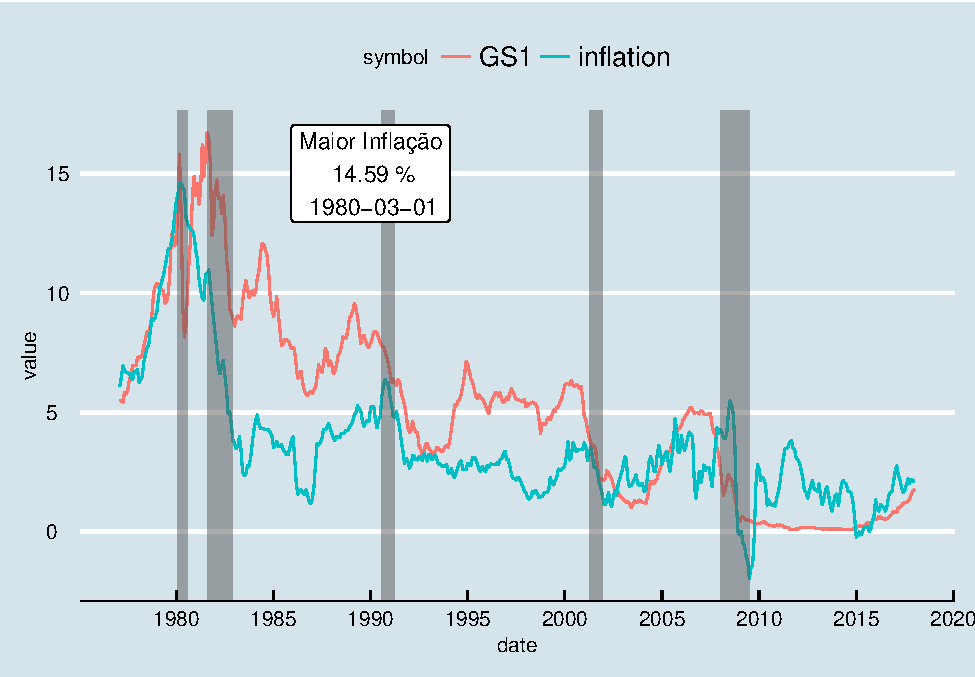
\includegraphics{Blanchar08-cap15_files/figure-latex/b_ggplot-1.pdf}
\caption{Inflação acumulada nos últimos 12 meses e taxa de juros
esperadas para o próximo ano. *Nota: áreas sombreadas indicam períodos
de recessão.}
\end{figure}

\begin{enumerate}
\def\labelenumi{\alph{enumi}.}
\setcounter{enumi}{2}
\tightlist
\item
  \emph{Para cada mês, calcule o spread entre as taxas de 30 anos e de 1
  ano. Plote no mesmo gráfico que a taxa de 1 ano.}
\end{enumerate}

vide Figura 2.

\begin{figure}
\centering
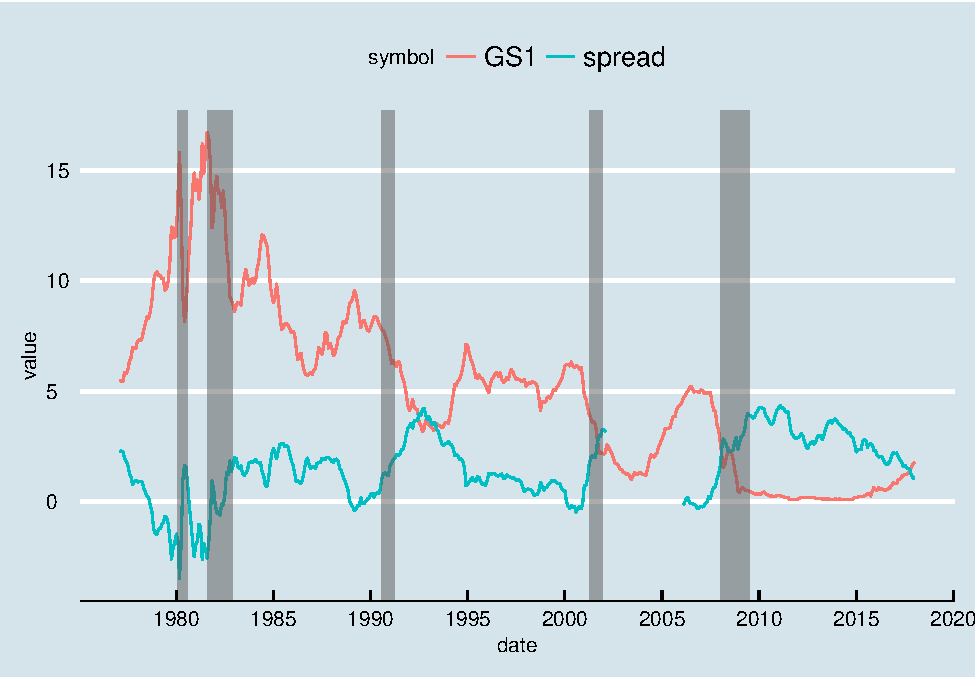
\includegraphics{Blanchar08-cap15_files/figure-latex/c_ggplot-1.pdf}
\caption{Spread entre as taxas de 30 anos e 1 ano e a própria taxa de 1
ano. *Nota: áreas sombreadas indicam períodos de recessão. **Nota: A
série de 30 anos de maturidade constante foi descontinuada em 18 de
fevereiro de 2002 e reintroduzida em 09 de fevereiro de 2006.}
\end{figure}

\begin{enumerate}
\def\labelenumi{\alph{enumi}.}
\setcounter{enumi}{3}
\tightlist
\item
  \emph{O que implica um spread declinante sobre as expectativas dos
  participantes do mercado financeiro? Enquanto a inflação esta subindo
  ao longo dos anos 70, o que estava ocorrendo com a taxa de 1 ano? Os
  participantes do mercado financeiro estavam esperando continuidade
  nesta tendência?}
\end{enumerate}

Enquanto a inflação aumentava, as taxas de juros de 1 ano também estavam
se elevando de acordo.

A partir do momento em que o spread se torna negativo, pode-se afirmar
que os participantes do mercado financeiro esperam uma queda nas taxas
de juros de curto prazo. Como estas quedas vêm acompanhadas de recessões
econômicas, podemos inferir que o mercado esperava uma recessão já antes
de 1980.

Como o mercado já estava esperando uma queda nas taxas curtas, não
podemos dizer que os participantes esperavam que esta tendência de alta
nos juros iria perdurar por muito mais tempo.

\begin{enumerate}
\def\labelenumi{\alph{enumi}.}
\setcounter{enumi}{4}
\tightlist
\item
  \emph{Utilizando o spread calculado em c. para outubro de 1979, você
  encontra alguma evidência da interpretação que o FED estava
  comprometido a combater a inflação?}
\end{enumerate}

Sim, em outubro de 1979 o spread entre a taxa de 30 anos e a taxa de 1
ano era de -2.59\% o que configura a inversão da curva de rendimentos. A
inversão desta curva sinaliza que os participantes do mercado esperam,
além de uma recessão futura, uma redução da inflação que será
acompanhada por redução nas taxas de juros de curto prazo.

\begin{enumerate}
\def\labelenumi{\alph{enumi}.}
\setcounter{enumi}{5}
\tightlist
\item
  \emph{Qual foi o efeito da política monetária expansionista adotada
  entre abril e julho de 1980 nas taxas de juros de 1 ano?}
\end{enumerate}

Esta troca na condução da política monetária resultou em rápida redução
nas taxas de curto prazo, como pode ser visto na Figura 2.

\begin{enumerate}
\def\labelenumi{\alph{enumi}.}
\setcounter{enumi}{6}
\tightlist
\item
  \emph{De abril a julho de 1980, os mercados esperavam que esta queda
  nas taxas de juros de curto prazo se manteriam? Estas expectativas
  estavam corretas?}
\end{enumerate}

No mesmo momento em que o FED adotou a política monetária expansionista,
o spread entre as taxas subitamente voltou ao terreno positivo, portanto
a curva de rendimentos voltou a estar positivamente inclinada. Uma curva
de rendimentos positivamente inclinada sinaliza expectativas de
\textbf{aumento} das taxas de juros pelo mercado. Desta forma, não, o
mercado não esperava que as taxas de juros de curto prazo se manteriam
baixas por muito tempo. Estas expectativas se demonstraram corretas,
pois logo depois o FED foi obrigado a novamente elevar suas taxas para
combater a inflação e o spread novamente mergulhou para valores
negativos.


\end{document}
